\newcommand\todo[1]{\textcolor{red}{#1}}
\chapter{Introduction}
\section{Act-R}


ACT-R, acronym of Adaptive Control of Thought-Rational, is a cognitive architecture: it is the implementation of a theory about how human cognition works. 
The aim of \mbox{ACT-R} is to model the behaviour of the human brain. From an external point of view \mbox{ACT-R} can be intended as a programming language; however its internal structure is based on assumptions about human cognition. The assumptions are established, through numerous experiments, by psychologists who research and study the human cognition,  ~\cite{Allen94}. 

A feature that distinguishes \mbox{ACT-R} from other theories in the field is the ability to collect quantitative measures that can be directly compared with those measures obtained from human participants. \todo{la prossima frase fa schifo}
The traditional measures of cognitive psychology, and so of \mbox{ACT-R}, are: time needed to perform the task, accuracy of the task and neurological data. For each task the researchers write models (programs) in \mbox{ACT-R}, adding their own assumptions related to it. 
A model simulates the behaviour of a cognitive agent. The approach, based on measuring and comparison, leads to very effective models, for example it has been shown that \mbox{ACT-R} can successfully predict \emph{Blood-Oxygen-Level Dependence (BOLD)} of several parts of the brain, through experiments with \emph{Functional Magnetic Resonance Imaging (fMRI)}.
Up to now \mbox{ACT-R} has been used successfully to create models in many different areas, the most important of witch are: learning, problem solving, communication and perception.

\mbox{ACT-R's} most important assumption is that human knowledge can be divided into two irreducible kinds of representations: declarative and procedural.
Declarative memory refers to all the kind of memory that can be consciously recalled, like the shape of an object or its color. Procedural memory is, instead, very different from the declarative one: it is referred to actions that can be done unconsciously. The most common way, used to explain how these two kind of memory work, is the typewriter example.
A skilled typewriter can write quickly without looking at the keyboard, putting his fingers in the right place and pushing them, in the correct order. If we ask to the same typewriter where a certain character is positioned in the keyboard, he will probably answer that he is not sure about that without looking at it. In this example the procedural memory is stored as the action of putting the right finger in the right place when the typewriter has the goal to write a certain character.

In \mbox{ACT-R} theory the declarative memory is represented by the so called \emph{chunks}, data structures defined as a n-tuple (slots) of arbitrary size. The n-tuples and their values are specified in the \emph{chunk-type}, it defines also (if any) the initial value of the slot. Every chunk has also a name, used to reference it, but that is not considered to be a part of the chunk itself. The chunks and their slots are used to implement the mechanisms of \mbox{ACT-R's} theory, even if the slots are only software construct and not part of the theory itself. The chunk-types can be organized in hierarchy.

The \mbox{ACT-R's} counter part of the human procedural memory are the \emph{productions}. Productions are the \mbox{ACT-R} equivalent of functions, they define sequences of actions and can be fired only if a set of preconditions are satisfied. 



All the activities carried out by the brain, i.e. talking or moving, are performed by neurons located close together, in a well defined and limited area of the cortex. Similarly each module of \mbox{ACT-R} represents a function of the human brain. In the \mbox{ACT-R's architecture} the task of the procedural module is to coordinate all the other modules. The exchange of information between the modules is achieved through \emph{buffers}.

\begin{figure}[h]
\begin{center} 
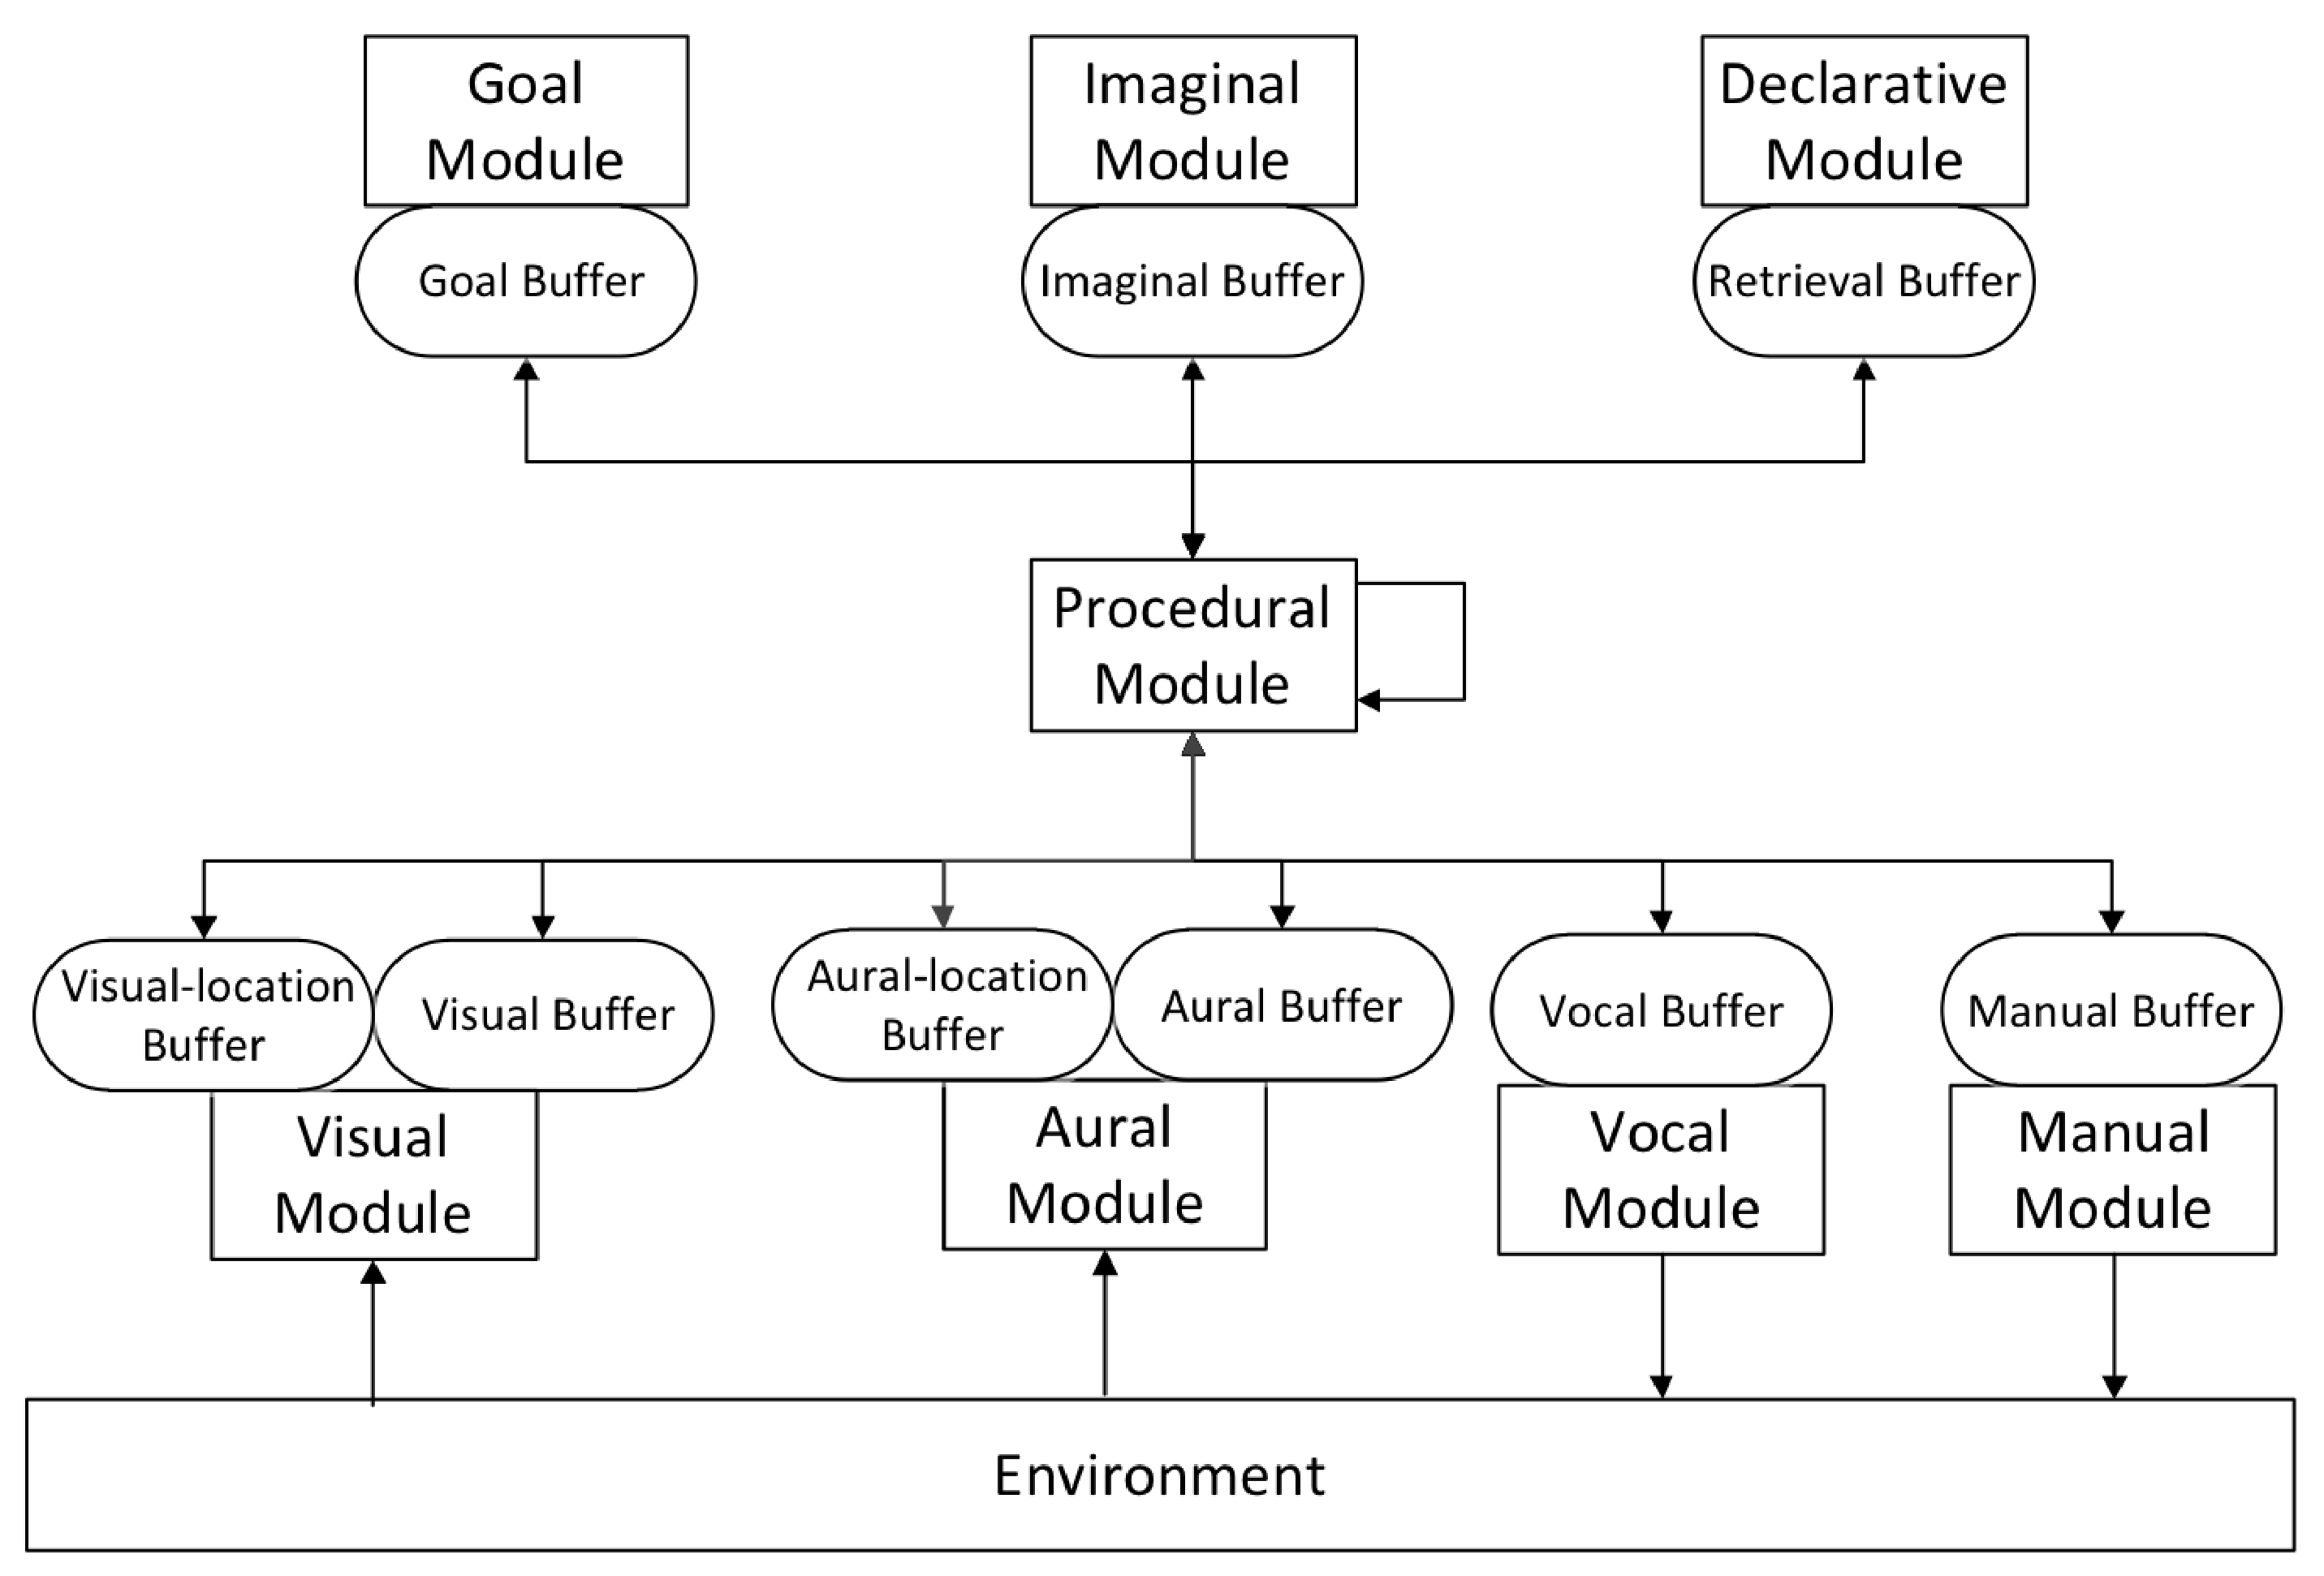
\includegraphics[scale=0.25]{images/01-img/actr.eps}
\end{center} 
\caption{\textit{Structure of Act-r.}}  
\label{fig:modulesActr}
\end{figure}

Each module is independent from the others, to communicate one to each other they need to pass through the procedural module. As shown in Figure  ~\ref{fig:modulesActr} a module can have more than one buffer, for example the aural module has two buffers: one is the "Aural-location Buffer", whose function is to get the focus about changes happened in the environment; the second is the "Aural Buffer", to get the real information about the environment.

The buffers are the built in interface between modules, used to exchange chunks between them. Every buffer belongs to a module, while a module can also have no buffers. Each buffer can hold one chunk at a time, which is readable by the other modules, the guidelines say that a buffer can be written only by its owner. 

Although the modules could work in parallel, their interaction is limited to a serial exchange of chunks. The modules usually work in a parallel way, but their interaction is only serial. There are two reasons for this limitation: firstly the structure of the buffers, can hold only one chunk; secondly only one production which preconditions are satisfied can be fired. When the preconditions of more than one production are satisfied the one to be fired is the one with the higher \emph{utility value}. This is a numeric quantity, it can be associated with each production in advance or it can be learned while the model runs.



From an informatics point of view \mbox{ACT-R} is a software written in Lisp and its models are written in a Lisp-like language. It is thought to have a modular structure so that it can be easily extended. \mbox{ACT-R 6.0} is the implementation of a state of the ars theory of human cognition, developed by John R. Anderson. Anderson credits Allen Newell as source of influence to his theory.
\newpage
\section{OpenCV}
\section{The objective}
The objective of this work is to control a mobile robot through the \mbox{ACT-R} framework. The robot will be able to navigate in real unknown environment and to find an object. The most important sensors used by the robot will be a \mbox{web-cam} and the bumpers. The data acquired from the \mbox{web-cam} will be used to improve the estimations of the actual position made with odometry. For example it will use information like perspective lines to be able to move in a corridor.
To achieve this goal a software layer is needed to enable the communication between ACT-R and the \mbox{web-cam}. The environment will have some requirements: it will be a relatively small place, like one or more than one room with flat floor, this due to the limited capability of movement of the robot, and it has to be mostly static. In the environment will be placed some \mbox{QR code}, used as landmarks. Those landmarks will be used to orientate easier in the environment.
The robot should also be able to avoid slow moving objects. From this point of view the robot will be a reactive agent, able to change its planning while the world near it changes. \todo{Cosa altro?}







